\documentclass[conference]{IEEEtran}
\usepackage{hyperref}
% *** GRAPHICS RELATED PACKAGES ***
%
\ifCLASSINFOpdf
   \usepackage[pdftex]{graphicx}
  % declare the path(s) where your graphic files are
  % \graphicspath{{../pdf/}{../jpeg/}}
  % and their extensions so you won't have to specify these with
  % every instance of \includegraphics
  % \DeclareGraphicsExtensions{.pdf,.jpeg,.png}
\else
  % or other class option (dvipsone, dvipdf, if not using dvips). graphicx
  % will default to the driver specified in the system graphics.cfg if no
  % driver is specified.
  % \usepackage[dvips]{graphicx}
  % declare the path(s) where your graphic files are
  % \graphicspath{{../eps/}}
  % and their extensions so you won't have to specify these with
  % every instance of \includegraphics
  % \DeclareGraphicsExtensions{.eps}
\fi


% correct bad hyphenation here
\hyphenation{op-tical net-works semi-conduc-tor}


\begin{document}
%
% paper title
% can use linebreaks \\ within to get better formatting as desired
\title{Time Series Data Mining Tool}


% author names and affiliations
% use a multiple column layout for up to three different
% affiliations
\author{\IEEEauthorblockN{Samir Sheriff}
\IEEEauthorblockA{Computer Science and Engineering\\
RV College of Engineering\\
Bangalore.\\
Email: samiriff@gmail.com}
\and
\IEEEauthorblockN{Satvik Neelakant}
\IEEEauthorblockA{Computer Science and Engineering\\
RV College of Engineering\\
Bangalore.\\
Email: nsatvik@gmail.com}
\and
\IEEEauthorblockN{Vaishakh BN}
\IEEEauthorblockA{Computer Science and Engineering\\
RV College of Engineering\\
Bangalore.\\
Email: vaishakhbn@gmail.com}
}

% conference papers do not typically use \thanks and this command
% is locked out in conference mode. If really needed, such as for
% the acknowledgment of grants, issue a \IEEEoverridecommandlockouts
% after \documentclass

% for over three affiliations, or if they all won't fit within the width
% of the page, use this alternative format:
% 
%\author{\IEEEauthorblockN{Michael Shell\IEEEauthorrefmark{1},
%Homer Simpson\IEEEauthorrefmark{2},
%James Kirk\IEEEauthorrefmark{3}, 
%Montgomery Scott\IEEEauthorrefmark{3} and
%Eldon Tyrell\IEEEauthorrefmark{4}}
%\IEEEauthorblockA{\IEEEauthorrefmark{1}School of Electrical and Computer Engineering\\
%Georgia Institute of Technology,
%Atlanta, Georgia 30332--0250\\ Email: see http://www.michaelshell.org/contact.html}
%\IEEEauthorblockA{\IEEEauthorrefmark{2}Twentieth Century Fox, Springfield, USA\\
%Email: homer@thesimpsons.com}
%\IEEEauthorblockA{\IEEEauthorrefmark{3}Starfleet Academy, San Francisco, California 96678-2391\\
%Telephone: (800) 555--1212, Fax: (888) 555--1212}
%\IEEEauthorblockA{\IEEEauthorrefmark{4}Tyrell Inc., 123 Replicant Street, Los Angeles, California 90210--4321}}




% use for special paper notices
%\IEEEspecialpapernotice{(Invited Paper)}




% make the title area
\maketitle


\begin{abstract}
%\boldmath
A time series is a sequence of data points, measured typically at successive points in time spaced at uniform time intervals. Time series analysis comprises methods for analyzing time series data in order to extract meaningful statistics and other characteristics of the data.In the context of statistics,the primary goal of time series analysis is forecasting. In the context of signal processing it is used for signal detection and estimation, while in the context of data mining, pattern recognition and machine learning time series analysis can be used for clustering, classification, query by content, anomaly detection as well as forecasting. This project is aimed making a time series data mining tool which can be used to accomplish the above goals. 



The tool developed can be used to perform anomaly detection, forecasting, similarity detection. The tool has been developed and tested using these data sets.

\end{abstract}
% IEEEtran.cls defaults to using nonbold math in the Abstract.
% This preserves the distinction between vectors and scalars. However,
% if the conference you are submitting to favors bold math in the abstract,
% then you can use LaTeX's standard command \boldmath at the very start
% of the abstract to achieve this. Many IEEE journals/conferences frown on
% math in the abstract anyway.

% no keywords

\begin{keywords}
time series, forecasting, similarity detection, anomaly detection.
\end{keywords}


% For peer review papers, you can put extra information on the cover
% page as needed:
% \ifCLASSOPTIONpeerreview
% \begin{center} \bfseries EDICS Category: 3-BBND \end{center}
% \fi
%
% For peerreview papers, this IEEEtran command inserts a page break and
% creates the second title. It will be ignored for other modes.
\IEEEpeerreviewmaketitle



\section{Introduction}
% no \IEEEPARstart
A time series is a set of observations $X_t$ , each one being recorded at a specific time t. Discrete-time time series is one in which the set T of times at which observations are made is a discrete set. Continuous-time time series are obtained when observations are recorded continuously over some time interval, e.g., when $T_0$ belongs [0,1]. Examples of time series are the daily closing value of the ECG readings and the annual flow volume of the Nile River at Aswan. Time series are very frequently plotted via line charts. Time series analysis comprises methods for analyzing time series data in order to extract meaningful statistics and other characteristics of the data. Time series forecasting is the use of a model to predict future values based on previously observed values.  
\begin{figure}[h!]
	\centering
		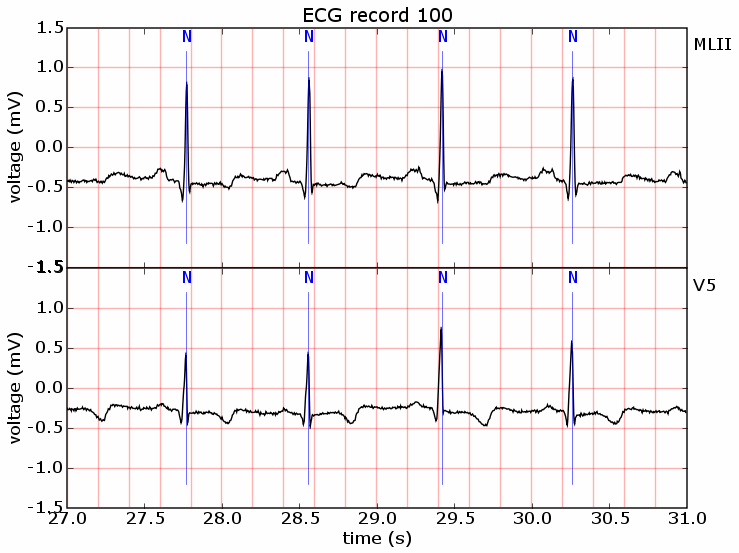
\includegraphics[scale=0.35]{screenshots/ecg.png}
		\caption{Time Series Example: ECG}
\end{figure}


\subsection{Literature Survey}
A time series is a collection of observations made sequentially through time. At each time point one or more measurements may be monitored corresponding to one or more attributes under consideration. The resulting time series is called univariate or multivariate respectively. In many cases the term sequence is used in order to refer to a time series, although some authors refer to this term only when the corresponding values are non-numerical. Throughout this paper the terms sequence and time series are being used interchangeably.
The most common tasks of time series data mining methods are: indexing, clustering, classification, novelty detection, motif discovery and rule discovery. In most of the cases, forecasting is based on the outcomes of the other tasks. A brief description of each task is given below.\\
\textbf{Indexing:} Find the most similar time series in a database to a given query time series.\\
\textbf{Clustering:} Find groups of time series in a database such that, time series of the same group are similar to each other whereas time series from different groups are dissimilar to each other.\\
\textbf{Classification:} Assign a given time series to a predefined group in a way that is more similar to other time series of the same group than it is to time series from other groups.\\
\textbf{Novelty detection:} Find all sections of a time series that contain a different behavior than the expected with respect to some base model.\\
\textbf{Motif discovery:} Detect previously unknown repeated patterns in a time series database.\\
\textbf{Rule discovery:} Infer rules from one or more time series describing the most possible behavior that they might present at a specific time point (or interval).\\




The ability to model and perform decision modeling and analysis is an essential feature of many real-world applications ranging from emergency medical treatment in intensive care units to military command and control systems. Existing formalisms and methods of inference have not been effective in real-time applications where trade-offs between decision quality and computational tractability are essential. The objective of this project is to fill the void that exists and help in proper analysis of time varying data.

\subsection{SCOPE}
The scope of a time series data mining tool is two fold. The first  is to obtain an understanding of the underlying forces and structure that produced the observed data. The second is to 
fit a model and proceed to forecasting, monitoring or even feedback and feed forward control. The time series data mining tool can be used in the following fields. 
\begin{itemize}
\item{\textbf{Economic Forecasting}}
\item{\textbf{Sales Forecasting}}
\item{\textbf{Rainfall Analysis}}
\item{\textbf{Stock Market Analysis}}
\item{\textbf{Yield Projections}}
\item{\textbf{Process and Quality Control}}
\item{\textbf{Census Analysis}}
\end{itemize}

\subsection{METHODOLOGY}
Time series analysis of data requires the user to able to view the different algorithms and the result obtained from each algorithm along with the graphs which help the user understand the time varying nature of the data. Hence, the representation of data becomes very important. Having understood this requirement in the early phase of the project, we adopted a methodology that will accomplish the objectives in a neat and intuitive way. A GUI was developed in the form of Java Server Pages and the back end was coded in Java which helped us exploit the object oriented paradigm in design of algorithms. 


\section{Software Requirements Specification}
Software Requirement Specification (SRS) is an important part of software development process. It includes a set of use cases that describe all the interactions of the users with the software. Requirements analysis is critical to the success of a project.
\subsection{Assumptions and Dependencies}
 \begin{itemize}
\item{}It is assumed that the user of this tool has basic understanding of time series data mining.
 
\item{}Also, the user must have a decent knowledge of the interpretation of line graphs.
\end{itemize}

\subsection{Specific Requirements}
This section shows the functional requirements that are to be satisfied by the system. All the requirements exposed here are essential to run this tool successfully.

\subsection{Functional Requirements}
\paragraph{}The functionality requirements for a system describe the functionality or the services that the system is expected to provide. This depends on the type of software system being developed. 
The requirements that are needed for this project are :
 \begin{itemize}
\item The data sets should be normalized so that the algorithms can be applied effectively.
\item A good representation of the results should be made available to the users through proper representation media like graphs.
\end{itemize}
 \subsection{Software Requirements}
\subsubsection{DEVELOPERS MACHINE}
\begin{itemize}
\item{	Operating System: Windows 7/8, Linux, Mac}
\item{  Software Tools : Java, JDK 7.0, Apache Tomcat Server version 7.0\\ Web Browser (Mozilla, IE8+, Chrome)} 
\item {IDE : Eclipse IDE for J2EE Developers}
\item {API Libraries : }JQuery UI and Ajax Libraries (Active Internet Connection)

\end{itemize}
\subsubsection{END USERS MACHINE}
\begin{itemize}
\item {Java Enabled Browser }
\item { Active Internet Connection }
\end{itemize}
\subsection{HARDWARE REQUIREMENTS}
\begin{itemize}
\item{Processor: Intel Pentium 4 or higher version}
\item{RAM: 512MB or more}
\item{Hard disk: 5 GB}
\end{itemize}
\subsubsection{SOFTWARE INTERFACES }
The Java Runtime Environment (JRE) is required to run the software.



\section{SYSTEM ARCHITECTURE}
This section provides an overview of  the functionality and the working of the time series data mining tool. The overall functionality of the application is divided into different modules in an efficient way. The system architecture is shown in Figure 2


\begin{figure}[h!]
	\centering
		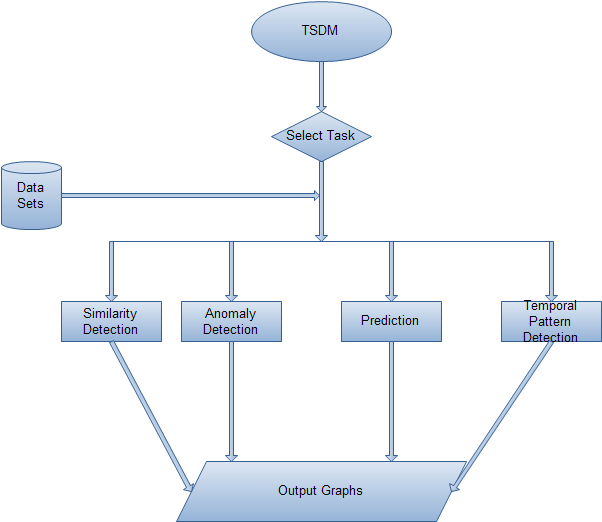
\includegraphics[scale=0.6]{system-architecture.png}
		\caption{System Architecture}
\end{figure} 

\subsection{DATA FLOW DIAGRAMS}
A DFD is a figure which shows the flow of data between the different processes and how the data is modified in each of the process. It is very important tool in software engineering that is used for studying the high level design.\\




There are many levels of DFDs. Level 0 gives the general description and level 1 gives the detailed description. Going higher in the level numbers greater description of the processes will be given.




\subsection{DFD LEVEL 0}
The level 0 DFD is shown in Fig. 3 below which gives the general operation of the TSDM Tool. There are two major components. One external entities called user and the TSDM Tool.
\begin{figure}[h!]
	\centering
		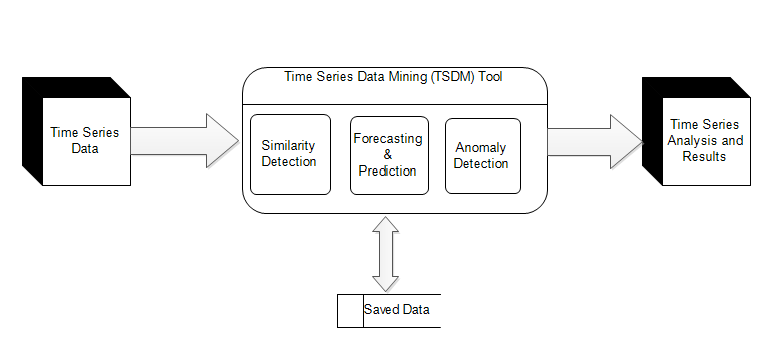
\includegraphics[scale=0.45]{screenshots/dfd_0.png}
		\caption{DFD Level 0}
\end{figure} 
\begin{itemize}
\item User : The User is the one responsible to send the data/instructions  to the TSDM Tool. The data may be a time series data or instructions to run datamining algorithms on the data.
\item TSDM Tool : This tool contains various algorithms implemented under different categories like similarity detection, forecasting, anomaly detection etc. Depending on the instructions sent by the user, the algorithms is run and the results are sent back.
\end{itemize}

\subsection{DFD Level 1}
The figure 4 shows the DFD level 1 diagram.
\begin{figure}[h!]
	\centering
		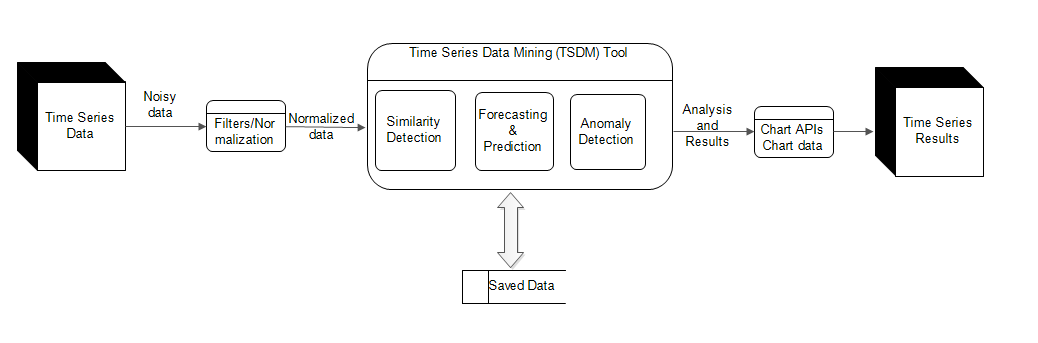
\includegraphics[scale=0.35]{screenshots/dfd_1.png}
		\caption{DFD Level 1}
\end{figure} 

\subsection{User Interaction Diagram}
The user interaction diagram in Figure 5 shows an overview of a user interacting with the TSDM Tool.
\begin{figure}[h!]
	\centering
		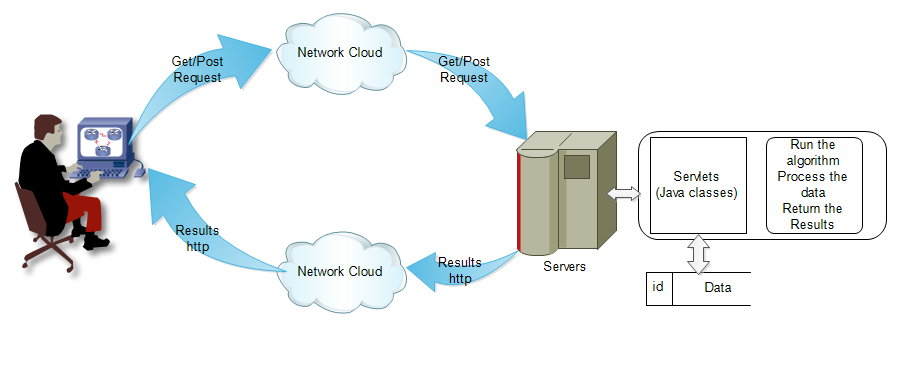
\includegraphics[scale=0.35]{screenshots/user_interaction.png}
		\caption{User Interaction Diagram}
\end{figure} 
\section{Implementation}
The implementation phase of any project development is the most important phase and yields the final solution which solves the problem at hand.The implementation phase involves the actual materialization of the ideas, which are expressed in a suitable programming language. The factors concerning the programming language selection and platform chosen are described in the following sections.


\subsection{Programming Language Selection}

\paragraph{}The programming language chosen must reflect the necessities of the project to be completely expressed in terms of the analysis and the design documents. Therefore before choosing the language, features to be included in the project are decided. The time series data mining project needs the following features in a language to be implemented. Some of the features required are stated as follows:
\begin{itemize}
\item J2EE provides us with servlets and JSP which help in dynamically constructing web pages.
\item J2EE provides us with Java Beans which help in proper data manipulation.
\item JSP and servlets make use of Java backend in a very optimal manner. They have special tags which help us exploit these features.
\item Java's core classes are designed from scratch to meet the requirements of an object oriented system.
\end{itemize} 
With these necessities in mind, J2EE is selected as the optimal programming language to implement the project.
\subsection{Platform}
\paragraph{}The TSDM tool was built and designed on Windows Operating system family. They were specifically tested on Windows 7 with Google Chrome and Mozilla Firefox browsers. Because the product is browser based, any user with the browsers mentioned above will be able to run the tool. The product is hence platform independent in the true sense.

\subsection{Modules}
This project is not yet complete and is currently under development. The description of the modules are below :
\begin{itemize}
\item \textbf{Similarity Detection} : This module helps in finding similarity patterns (that occur at regular intervals in case of periodic time series), comparing different time series data. SAX and DTW are the main algorithms implemented/used in this module.
\item \textbf{Forecasting and Prediction} : This module contain algorithms/models which can be trained from the past time series data and can be used to predict the future values of a time series. 
\item \textbf{Anomaly Detection} : This module contains algorithms that help in indicating anomalous patterns in the time series data analyzed. Anomalies are patterns in time series which deviate from the normal behavior and can indicate fraud/danger depending on the application. For example in an industry which produces the blades, the thickness of the blade can be monitored by a machine as a time series and any deviation from the normal error rate can signal an error in the manufacturing process.
\item \textbf{Temporal Pattern Finder } : This module helps in finding hidden temporal patterns in a time series. This module can be further extended to implement clustering techniques.
\end{itemize}

\section{Conclusion}
\subsection{Summary}
In this project, we were able to successfully implement the Time Series Data Mining Tool for analyzing the time series and test its performance. This tool mainly contains four modules, they are - \textbf{Similarity Detection, Forecasting and Prediction, Anomaly Detection and Temporal Pattern Finder}, which we were successful in implementing and testing. The results obtained were presented in the previous section.


Initially this project mainly focused on analyzing the sea and water level time series. Later this application was extended to any uni-variate time series data. Users can upload the time series data to be analyzed and get the results instantly. Major data sets used were :
\begin{itemize}
\item Sea Level Dataset : Indicating the sea level at various times of a day.
\item Water Level : Ground Water level data, indicating the ground water level during various moths of an year for upto 5 years.
\item Finance Dataset : Consisting of stock index values of  Nifty and Vix collected every minuted for a week.(5 days,during market hours).
\item ECG Dataset : The ECG  voltage values of patients collected every 4ms.(for 10 patients).
\end{itemize}


In this project, we also analyzed the efficiencies of different algorithms for the same tasks and also compared the results for different data sets.Clearly more work needs to be done.

\section{Future enhancements}
Some of the future enhancements are :
\begin{enumerate}
\item{The size of the  time series data analyzed is in terms of Mega Bytes. For larger dataset(In terms of GBs) or big data, distributed computing technologies like Hadoop can be used.}
\item{}The application can be extended to analyze multi variate time series data.
\item{The application could be made more responsive by using Threads and Parallel/Cloud Computing}
\item{One more extension could be analyzing twitter post data with respect to time and predicting the trends. This requires NLP, but is an example of time series.}
\item{Efficient algorithms using Support Vector Models (SVMs) for forecasting, Hidden Markov Model for anomaly detection can be implemented.}
\item{This application uses static time series data, enhancements can be made to use real time data.(In finance applications)}

\item{This application can be converted into an mobile application (android, iPhone, iPad) where the users can analyze the time series data on the go and share the results on facebook}

\end{enumerate}


% use section* for acknowledgement
\section*{Acknowledgment}
The authors wish to express their gratitude to \textbf{Dr. Shobha G. and Mrs. Shantha Rangaswamy}, who offered invaluable assistance, support and guidance
throughout the development of this tool.



% trigger a \newpage just before the given reference
% number - used to balance the columns on the last page
% adjust value as needed - may need to be readjusted if
% the document is modified later
%\IEEEtriggeratref{8}
% The "triggered" command can be changed if desired:
%\IEEEtriggercmd{\enlargethispage{-5in}}

% references section

% can use a bibliography generated by BibTeX as a .bbl file
% BibTeX documentation can be easily obtained at:
% http://www.ctan.org/tex-archive/biblio/bibtex/contrib/doc/
% The IEEEtran BibTeX style support page is at:
% http://www.michaelshell.org/tex/ieeetran/bibtex/
%\bibliographystyle{IEEEtran}
% argument is your BibTeX string definitions and bibliography database(s)
%\bibliography{IEEEabrv,../bib/paper}
%
% <OR> manually copy in the resultant .bbl file
% set second argument of \begin to the number of references
% (used to reserve space for the reference number labels box)
\begin{thebibliography}{1}

\bibitem{test}Agrawal R., Lin K.-I., Sawhney H. S., Shim K.,\textit{“Fast Similarity Search in the Presence of Noise,Scaling, and Translation in Time-Series Databases”}
\bibitem{t}Genetic Algorithm for constructing DT - \url{http://www.jprr.org/index.php/jprr/article/viewFile/44/25}
\bibitem{te}Decision Trees - \url{http://web.cecs.pdx.edu/~mm/MachineLearningWinter2010/pdfslides/DecisionTrees.pdf}
\bibitem{t} Project brief for the DT  using Horse data sets  - \url{https://cs.uwaterloo.ca/~ppoupart/teaching/cs486-spring06/assignments/asst4/asst4.pdf}
\bibitem{t}Supervised and Unsupervised Discretization of Continous Features - \url{http://robotics.stanford.edu/users/sahami/papers-dir/disc.pdf}
\bibitem{t}Naming Convention -\textit{Wikipedia} :  \url{http://en.wikipedia.org/wiki/Naming_convention_(programming)}
\bibitem{t}Code Conventions for the Java Programming Language - \url{http://www.oracle.com/technetwork/java/codeconv-138413.html}

\end{thebibliography}




% that's all folks
\end{document}


